\href{https://github.com/yassienE4/OS-VM/commit/b7e12deff3fbcc65242c960350334ebbc79c81e6}{\ul{https://github.com/yassienE4/OS-VM/commit/b7e12deff3fbcc65242c960350334ebbc79c81e6}}

How to run

\begin{itemize}
\item
  First make sure the python env is activated
\item
  ``source /workspaces/OS-VM/venv/bin/activate''
\item
  Second move to working directory
\item
  cd /workspaces/OS-VM/scheduling
\item
  ./run.sh main.cpp
\item
  The c++ code should automatically call the python plot script
\end{itemize}

How the code works:

First i created a DS to store each process, storing arrival time, burst
time, and a unique id

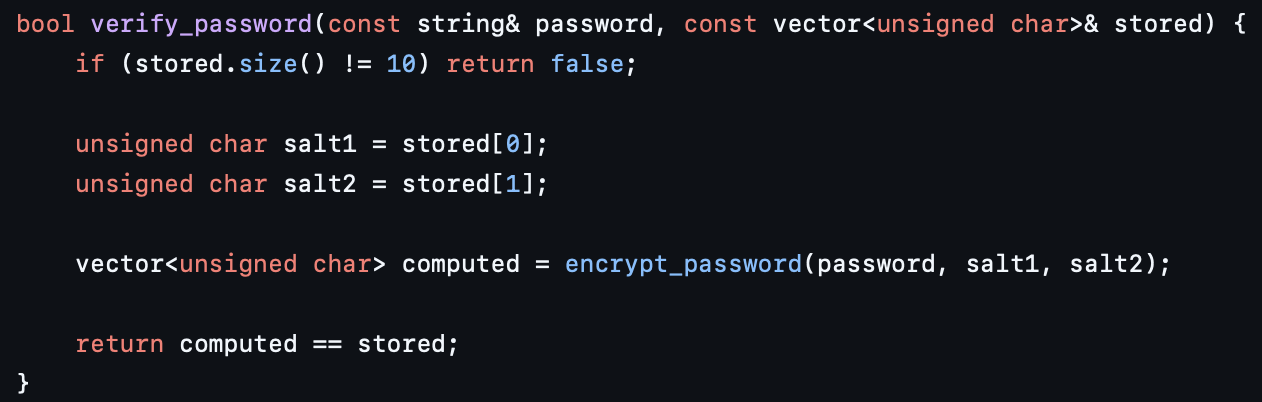
\includegraphics[width=3.10417in,height=2.10417in]{./images/media/image2.png}

In main, we read each process from the text file, and then call the
respective function for each algorithm

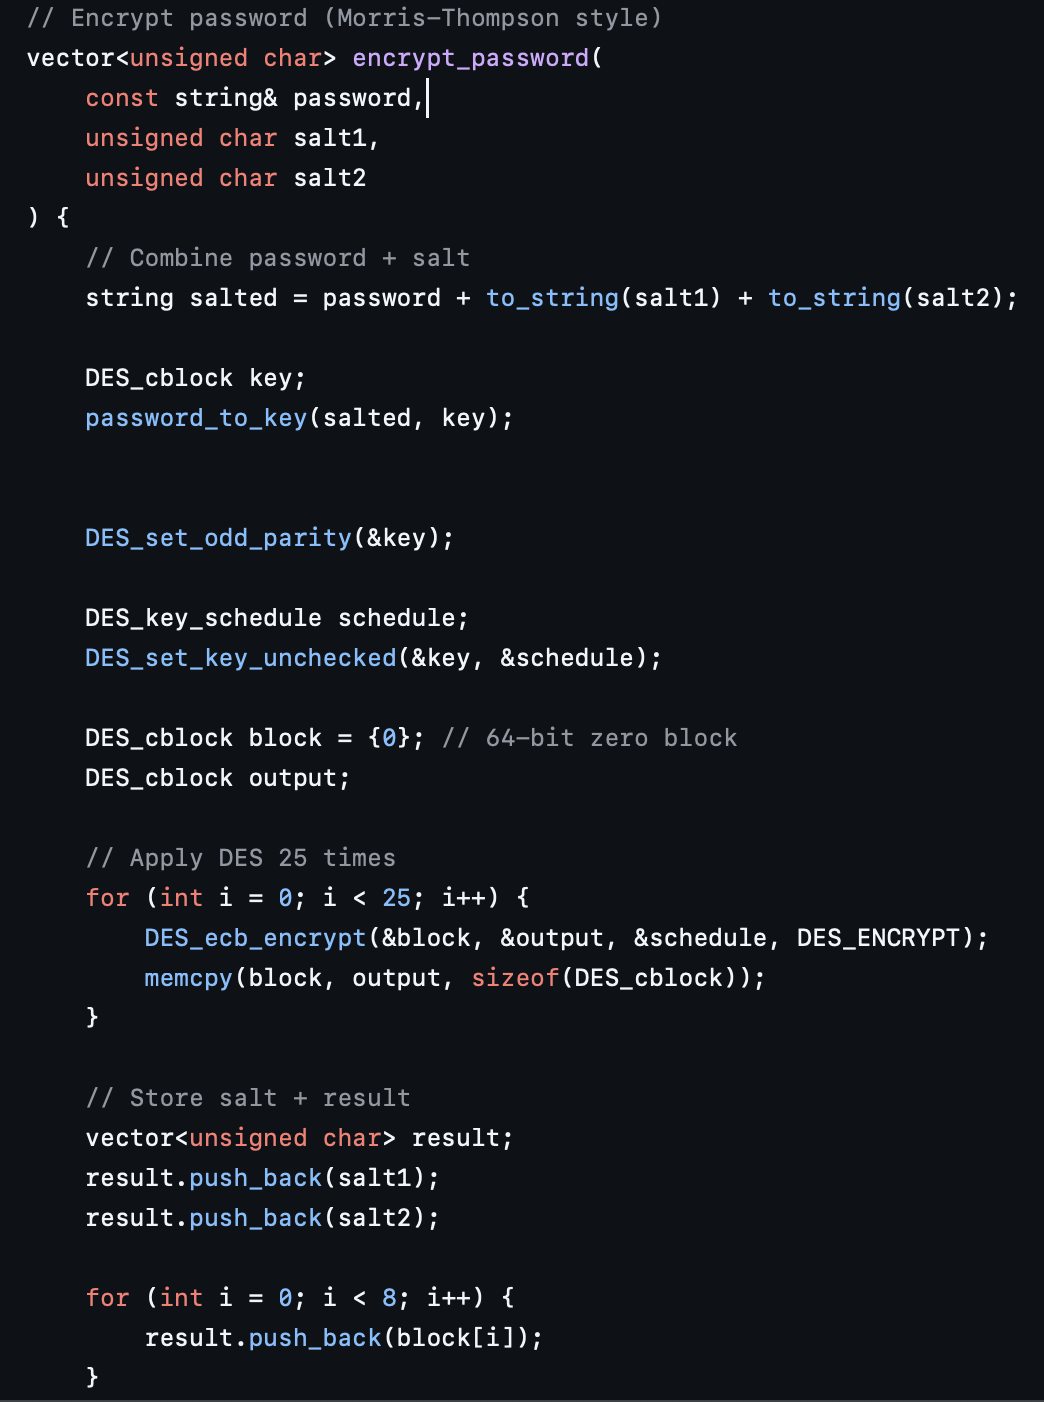
\includegraphics[width=4.83333in,height=4.60417in]{./images/media/image4.png}

For first come first serve

\begin{itemize}
\item
  We first sort our processes by arrival time
\item
  We simulate each process by

  \begin{itemize}
  \item
    First if its ``idle'', we simulate time passing
  \item
    We then compute waiting time by Waiting time = start time − arrival
    time
  \item
    Then ``execute'' the process by running the process for the full
    burst time
  \item
    Then return average waiting time
  \end{itemize}
\end{itemize}

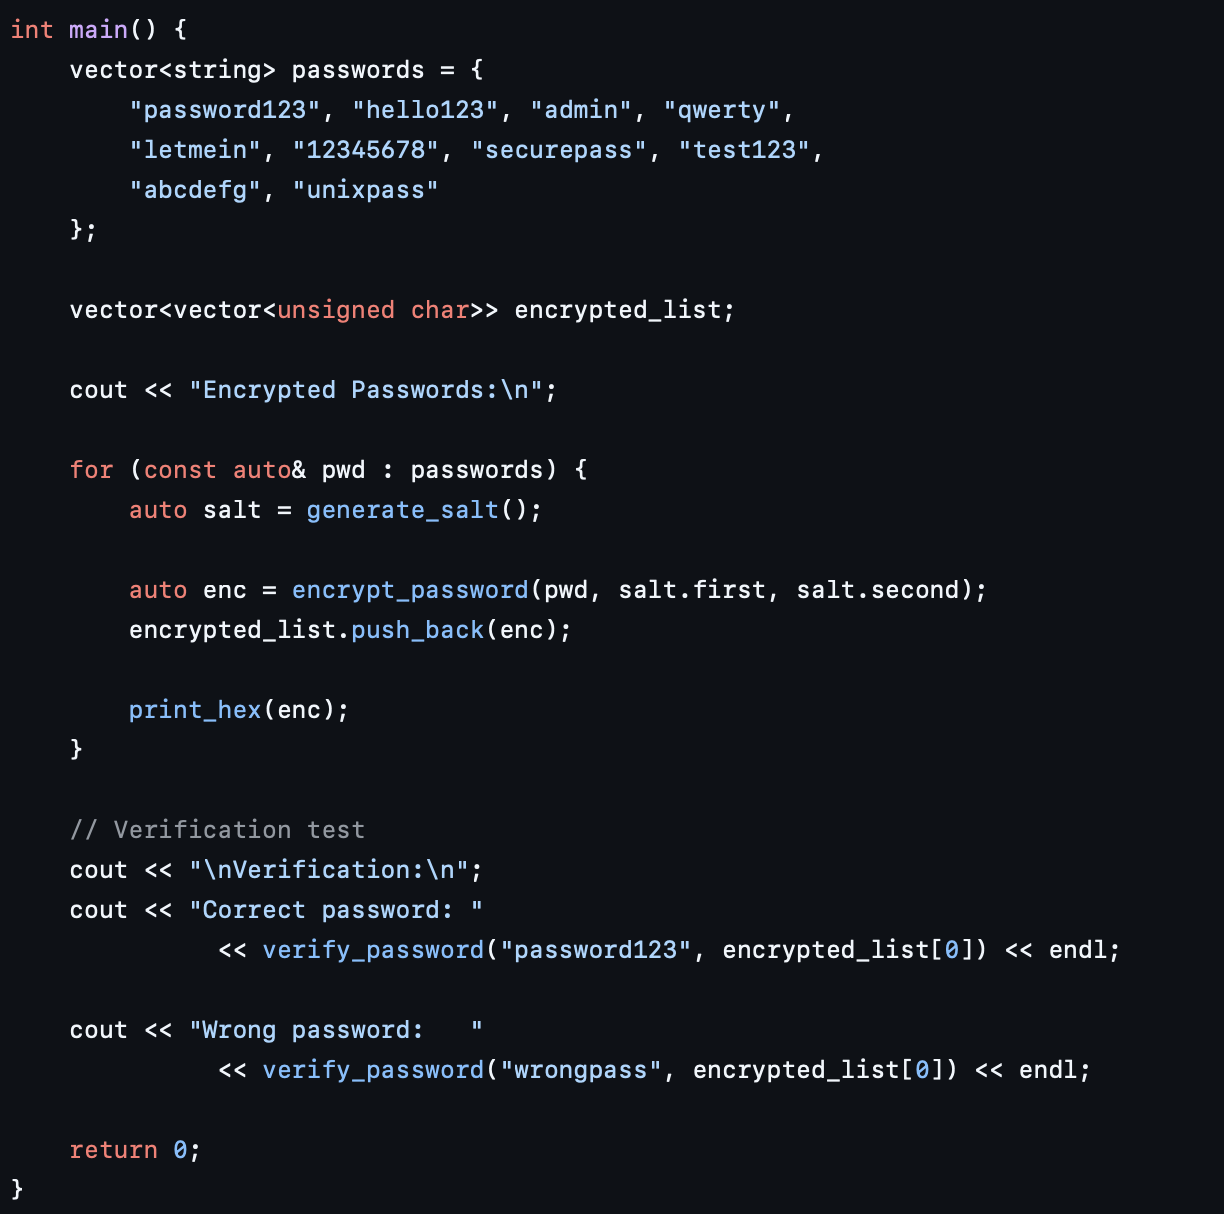
\includegraphics[width=6.5in,height=4.15278in]{./images/media/image3.png}

For SJF

\begin{itemize}
\item
  We find the shortest available process by
\item
  Scanning all processes and picking the unfinished process with:

  \begin{itemize}
  \item
    arrival \textless= current time
  \item
    smallest burst time
  \end{itemize}
\item
  If none is found we set index to -1, which is handled by simulating
  idle time
\item
  We then execute the process
\end{itemize}

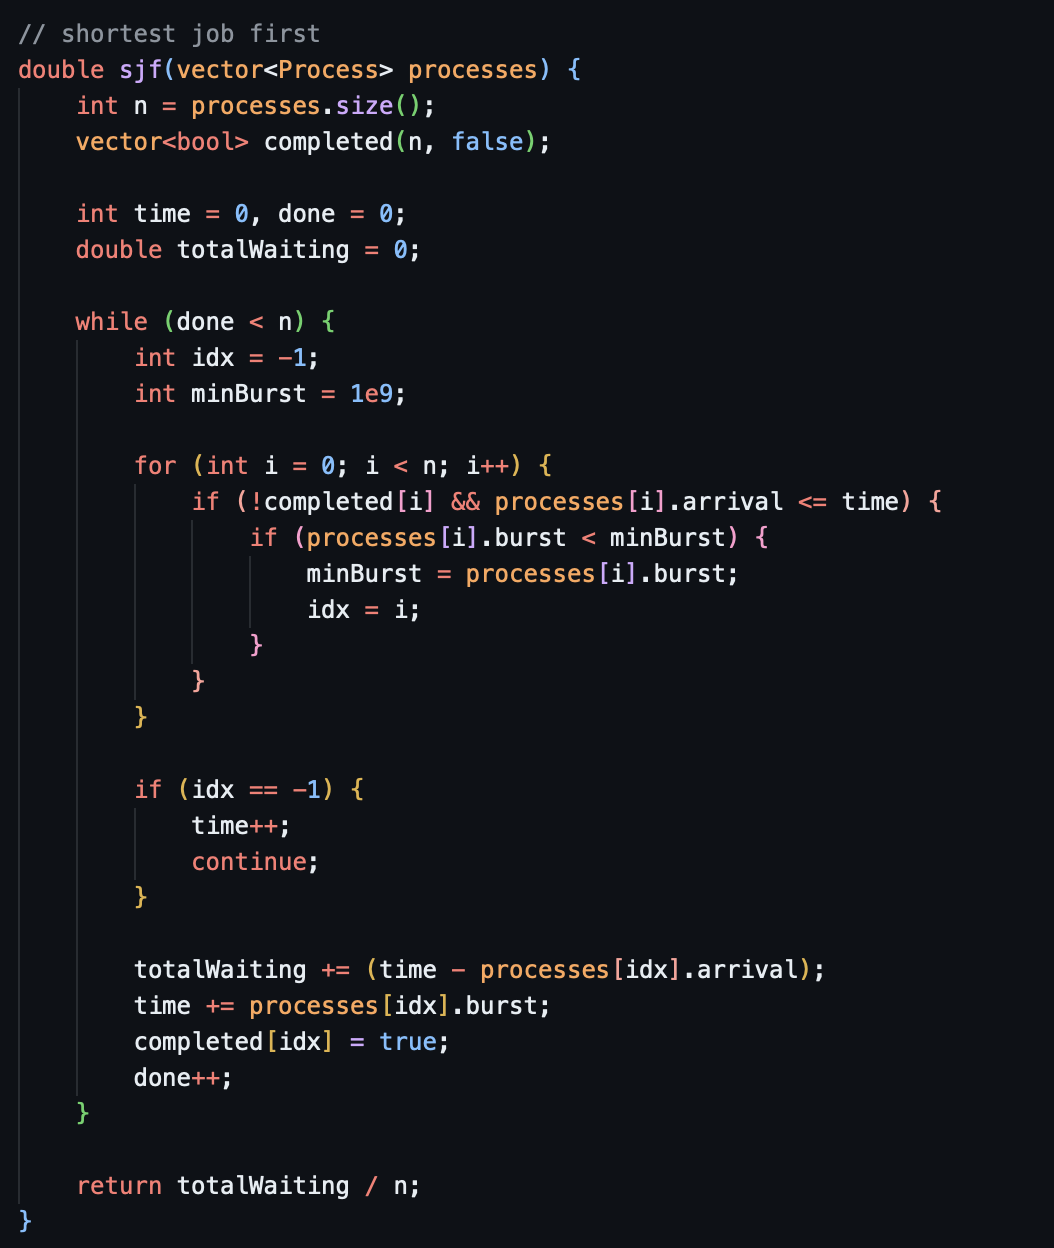
\includegraphics[width=5.66555in,height=6.70969in]{./images/media/image7.png}

For round Robin

\begin{itemize}
\item
  We initialize the queue, with ready processes
\item
  And an array with remaining burst time
\item
  We add process to queue if they meet arrival \textless= current time
\item
  If queue is empty = all current processes are executed, so we simulate
  time until we reach a process
\item
  We then choose the next process by taking the front of the queue
\item
  We then execute the process only for the chosen quantum time,
\item
  We then add newly arrived processes
\item
  We then handle the executed process
\item
  If it still has remaining time, we push it back to the queue
\item
  If not, we increment completed counter and update waiting time
\end{itemize}

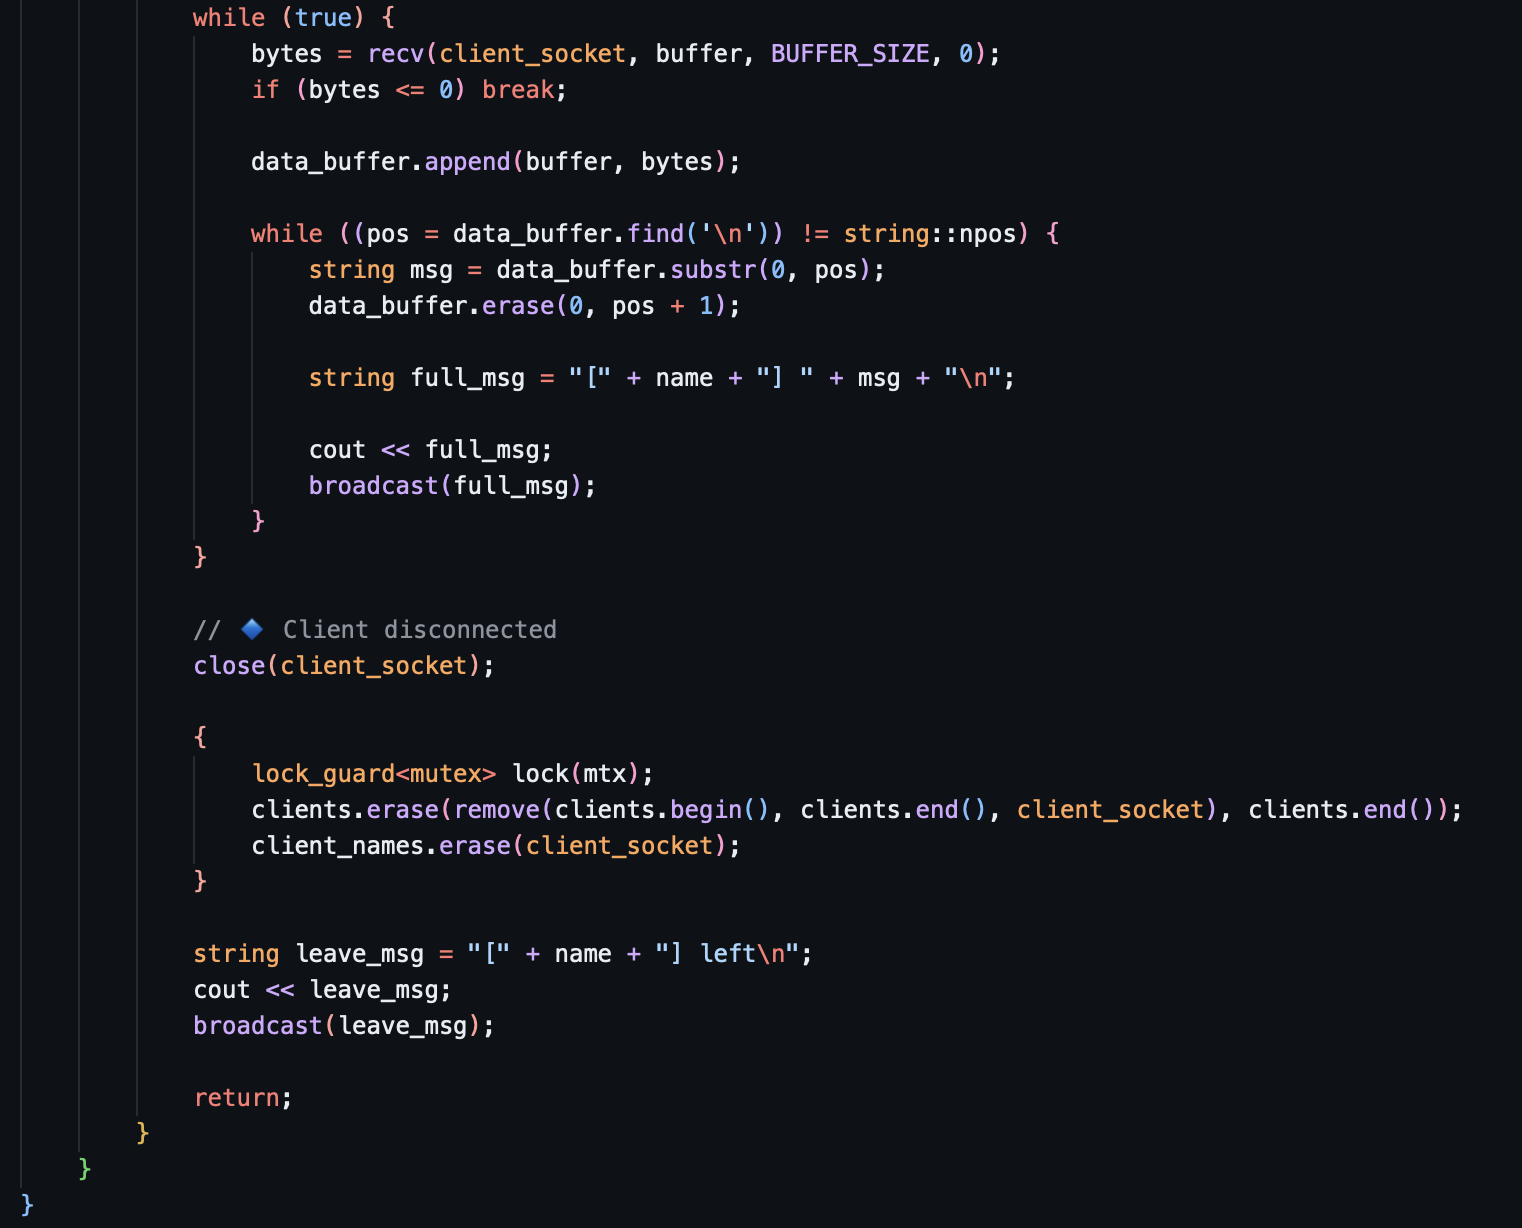
\includegraphics[width=4.3436in,height=6.48438in]{./images/media/image6.png}

Back in the main function:

\begin{itemize}
\item
  We output the average waiting times
\item
  And export as CSV
\item
  We then call a python script
\end{itemize}

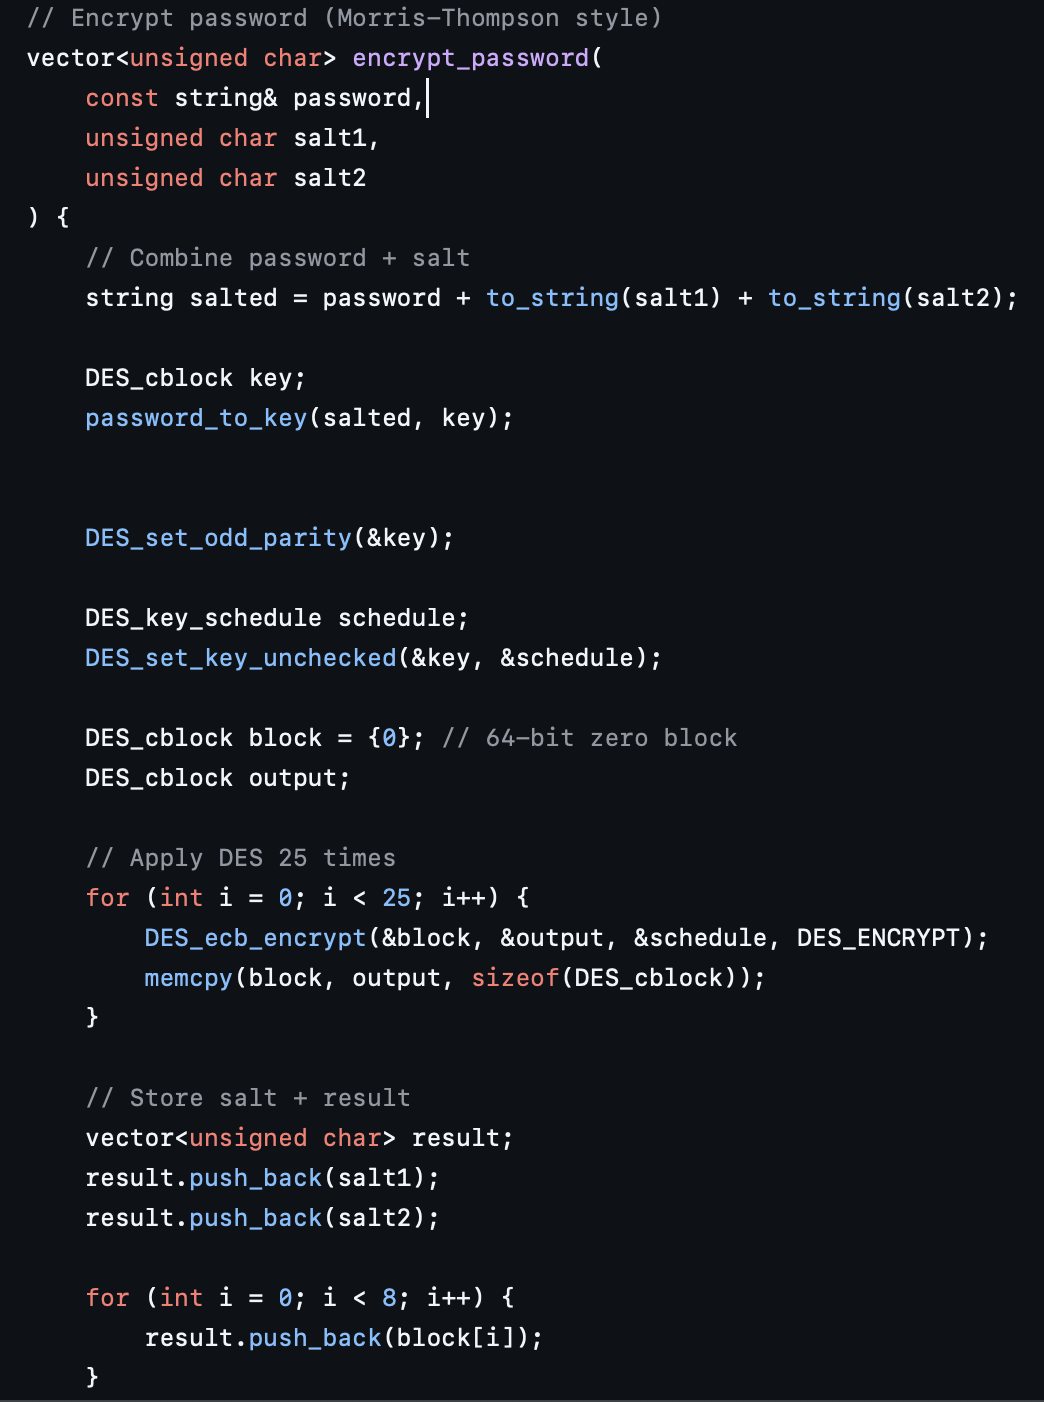
\includegraphics[width=4.83333in,height=4.76042in]{./images/media/image4.png}

In the python script, we parse the csv file and use matplotlib to create
a bar chart

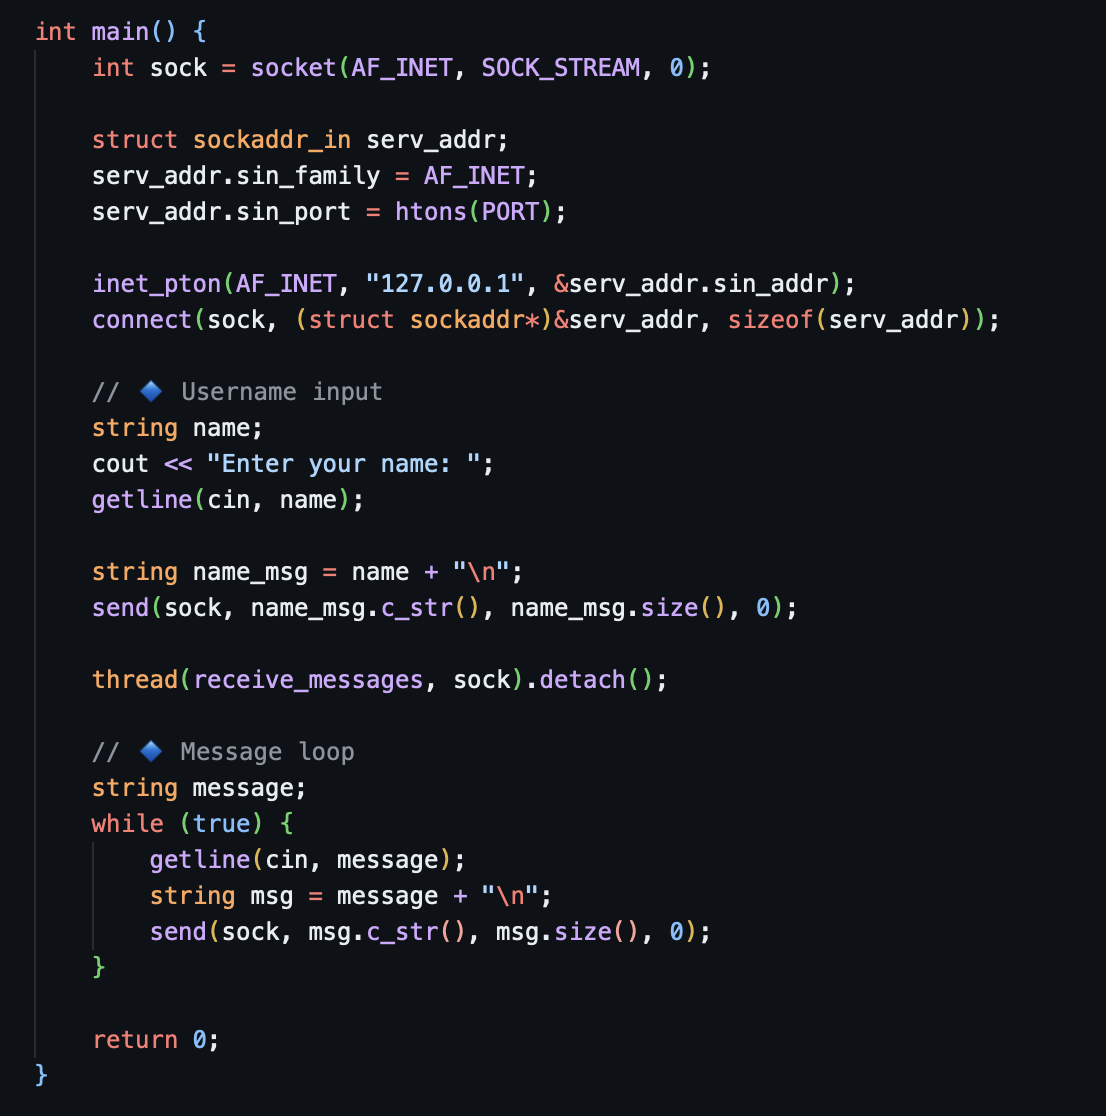
\includegraphics[width=6.5in,height=5.73611in]{./images/media/image5.png}

Findings:

With this text file setup

4 (number of processes)

0 5 ( arrival / burst)

1 3 ( arrival / burst)

2 8 ( arrival / burst)

3 6 ( arrival / burst)

2 (quantum time)

We get this output

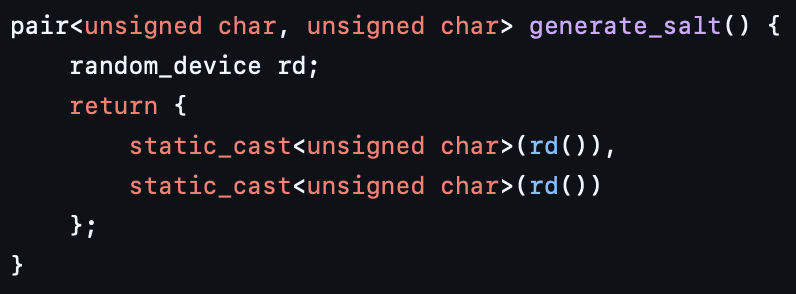
\includegraphics[width=4.39063in,height=3.28988in]{./images/media/image1.png}

Shortest job first has the lowest waiting time, as it focuses on
minimizing it

Round Robin maximizes fairness but as a result processes get interrupted
and waiting time goes up

FCFS is in between, but leans towards SJF more, as the processes are not
interrupted.
